\documentclass{article}

\usepackage{fancyhdr}
\usepackage{extramarks}
\usepackage{amsmath}
\usepackage{amsthm}
\usepackage{amsfonts}
\usepackage{tikz}
\usepackage[plain]{algorithm}
\usepackage{algpseudocode}
\usepackage{graphicx}
\usepackage{mcode}
\usetikzlibrary{automata,positioning}

%
% Basic Document Settings
%

\topmargin=-0.45in
\evensidemargin=0in
\oddsidemargin=0in
\textwidth=6.5in
\textheight=9.0in
\headsep=0.25in

\linespread{1.1}

\pagestyle{fancy}
\lhead{\hmwkAuthorName}
\chead{\hmwkClass\ (\hmwkClassInstructor\ \hmwkClassTime): \hmwkTitle}
\rhead{\firstxmark}
\lfoot{\lastxmark}
\cfoot{\thepage}

\renewcommand\headrulewidth{0.4pt}
\renewcommand\footrulewidth{0.4pt}

\setlength\parindent{0pt}

%
% Create Problem Sections
%

\newcommand{\enterProblemHeader}[1]{
    \nobreak\extramarks{}{Problem \arabic{#1} continued on next page\ldots}\nobreak{}
    \nobreak\extramarks{Problem \arabic{#1} (continued)}{Problem \arabic{#1} continued on next page\ldots}\nobreak{}
}

\newcommand{\exitProblemHeader}[1]{
    \nobreak\extramarks{Problem \arabic{#1} (continued)}{Problem \arabic{#1} continued on next page\ldots}\nobreak{}
    \stepcounter{#1}
    \nobreak\extramarks{Problem \arabic{#1}}{}\nobreak{}
}

\setcounter{secnumdepth}{0}
\newcounter{partCounter}
\newcounter{homeworkProblemCounter}
\setcounter{homeworkProblemCounter}{1}
\nobreak\extramarks{Problem \arabic{homeworkProblemCounter}}{}\nobreak{}

%
% Homework Problem Environment
%
% This environment takes an optional argument. When given, it will adjust the
% problem counter. This is useful for when the problems given for your
% assignment aren't sequential. See the last 3 problems of this template for an
% example.
%
\newenvironment{homeworkProblem}[1][-1]{
    \ifnum#1>0
        \setcounter{homeworkProblemCounter}{#1}
    \fi
    \section{Problem \arabic{homeworkProblemCounter}}
    \setcounter{partCounter}{1}
    \enterProblemHeader{homeworkProblemCounter}
}{
    \exitProblemHeader{homeworkProblemCounter}
}

%
% Homework Details
%   - Title
%   - Due date
%   - Class
%   - Section/Time
%   - Instructor
%   - Author
%

\newcommand{\hmwkTitle}{Homework\ \#3}
\newcommand{\hmwkDueDate}{October 28, 2016}
\newcommand{\hmwkClass}{STAT5444}
\newcommand{\hmwkClassTime}{12:20 MWF}
\newcommand{\hmwkClassInstructor}{Professor Scott Leman}
\newcommand{\hmwkAuthorName}{Kevin Malhotra}

%
% Title Page
%

\title{
    \vspace{2in}
    \textmd{\textbf{\hmwkClass:\ \hmwkTitle}}\\
    \normalsize\vspace{0.1in}\small{Due\ on\ \hmwkDueDate\ at 3:10pm}\\
    \vspace{0.1in}\large{\textit{\hmwkClassInstructor\ \hmwkClassTime}}
    \vspace{3in}
}

\author{\textbf{\hmwkAuthorName}}
\date{}

\renewcommand{\part}[1]{\textbf{\large Part \Alph{partCounter}}\stepcounter{partCounter}\\}

%
% Various Helper Commands
%

% Useful for algorithms
\newcommand{\alg}[1]{\textsc{\bfseries \footnotesize #1}}

% For derivatives
\newcommand{\deriv}[1]{\frac{\mathrm{d}}{\mathrm{d}x} (#1)}

% For partial derivatives
\newcommand{\pderiv}[2]{\frac{\partial}{\partial #1} (#2)}

% Integral dx
\newcommand{\dx}{\mathrm{d}x}

% Alias for the Solution section header
\newcommand{\solution}{\textbf{\large Solution}}

% Probability commands: Expectation, Variance, Covariance, Bias
\newcommand{\E}{\mathrm{E}}
\newcommand{\Var}{\mathrm{Var}}
\newcommand{\Cov}{\mathrm{Cov}}
\newcommand{\Bias}{\mathrm{Bias}}

\begin{document}

\maketitle

\pagebreak

\begin{homeworkProblem}
\begin{align*}
p(\mu | X) &= \int L(\mu, \Sigma | X) p(\mu) p(\Sigma) d\Sigma \\
p(\mu | X) &\propto \int \prod_{i=0}^N |\Sigma|^{-\frac{1}{2}} 
	e^{\frac{-1}{2}(X - \mu)^T\Sigma^{-1}(X - \mu)} |\Sigma|^{-\frac{k+1}{2}}\\
p(\mu | X) &\propto \int |\Sigma^{-1}|^{\frac{N+K+1}{2}} 
	e^{\sum_{i=0}^N \frac{-1}{2}(X_i - \mu)^T\Sigma^{-1}(X_i - \mu)}\\
p(\mu | X) &\propto \int |\Sigma^{-1}|^{\frac{N+K+1}{2}} 
	e^{\frac{-1}{2}Tr(\sum_{i=0}^N (X_i - \mu)(X_i - \mu)^T\Sigma^{-1})}\\
	\Sigma^{-1}&-InvWishart(\sum_{i=0}^N (X_i - \mu)(X_i - \mu)^T, N) \\
p(\mu | X) &\propto \int |\Sigma^{-1}|^{\frac{N+K+1}{2}} 
	e^{\frac{-1}{2}Tr(\sum_{i=0}^N (X_i - \mu)(X_i - \mu)^T\Sigma^{-1})}
	* \frac{
	\frac{|\sum_{i=0}^N (X_i - \mu)(X_i - \mu)^T|^{N/2}}{2^{\frac{NK}{2}}\Gamma_p(N/2)}}
	{\frac{|\sum_{i=0}^N (X_i - \mu)(X_i - \mu)^T|^{N/2}}{2^{\frac{NK}{2}}\Gamma_p(N/2)}}\\
p(\mu | X) &\propto
	\frac{2^{\frac{NK}{2}}\Gamma_p(N/2)}{|\sum_{i=0}^N (X_i - \mu)(X_i - \mu)^T|^{N/2}}\\
p(\mu | X) &\propto |\sum_{i=0}^N (X_i - \mu)(X_i - \mu)^T|^{-N/2}\\
p(\mu | X) &\propto 
	|\sum_{i=0}^N [(X_i - \bar{X})+(\bar{X} - \mu)][(X_i - \bar{X})+(\bar{X} - \mu)]^T|^{-N/2}\\
p(\mu | X) &\propto 
	|\sum_{i=0}^N (X_i - \bar{X})(X_i - \bar{X})^T +
					  (X_i - \bar{X})(\bar{X} - \mu)^T \\
					 &+ (\bar{X} - \mu)(X_i - \bar{X})^T +
					  (\bar{X} - \mu)(\bar{X} - \mu)^T|^{-N/2}\\
p(\mu | X) &\propto 
	|\sum_{i=0}^N (X_i - \bar{X})(X_i - \bar{X})^T + (\bar{X} - \mu)(\bar{X} - \mu)^T|^{-N/2}\\
	S^2 &= \frac{\sum_{i=0}^N(X_i - \bar{X})(X_i - \bar{X})^T}{N-K} \\
p(\mu | X) &\propto 
	|(N-K)S^2 + N(\bar{X} - \mu)(\bar{X} - \mu)^T|^{-N/2}\\ \\
	Sherman&-Morrison-Woodbury |A + XBX^T| = |A||B||B^T + X^TA^{-1}X|\\ \\
p(\mu | X) &\propto 
	\bigg(|(N-K)S^2||1+(\bar{X} - \mu)[(N-K)S^2]^{-1}(\bar{X} - \mu)^T|\bigg)^{-N/2}\\
p(\mu | X) &\propto |1+(\bar{X} - \mu)[(N-K)S^2]^{-1}(\bar{X} - \mu)^T|^{-(N-k+k)/2}\\
p(\mu | X) &\propto |1+\frac{N-k}{N-k}(\bar{X} - \mu)[(N-K)S^2]^{-1}(\bar{X} - \mu)^T|^{-(N-k+k)//2}\\
p(\mu | X) &\propto |1+\frac{1}{N-k}(\bar{X} - \mu)[(N-K)S^2]^{-1}(\bar{X} - \mu)^T|^{-(N-k+k)//2}\\
\mu &- t_{(N-k)} (\bar{X}, [(N-K)S^2]^{-1})
\end{align*}
\end{homeworkProblem}
\pagebreak
\begin{homeworkProblem}
Part 1: \\
\includegraphics[scale=0.4]{HW3_part1} \\
Part 2: \\
\includegraphics[scale=0.4]{HW3_part2} \\
\pagebreak
\lstinputlisting{HW3.m}
Part 3: \\
\begin{align*}
\mu &= (X^TX)^{-1}Y \\ 
\psi &= \sigma^2 (X^TX)^{-1} \\
\gamma &- Gamma(a, b) \\
\beta &-N(\mu, \frac{\psi}{\gamma}) \\
p(\beta|\mu, \psi) &= \int L(\beta|\mu, \psi, \gamma) p(\gamma) d\gamma \\
p(\beta|\mu, \psi) &\propto \int |\frac{\psi}{\gamma}|^{-1/2}
	e^{\frac{-1}{2}(\beta - \mu)^T|\frac{\psi}{\gamma}|^{-1}(\beta - \mu)} *
	\gamma^{a-1}e^{-b\gamma} d\gamma \\
p(\beta|\mu, \psi) &\propto \int |\psi|^{-1/2} \gamma^{\frac{1}{2} + a - 1}
	e^{\frac{-1}{2}(\beta - \mu)^T|\frac{\psi}{\gamma}|^{-1}(\beta - \mu)} *
	e^{-b\gamma} d\gamma \\
p(\beta|\mu, \psi) &\propto |\psi|^{-1/2} \int \gamma^{\frac{1}{2} + a - 1}
	e^{-\gamma\big(\big[\frac{1}{2}(\beta - \mu)^T|\psi|^{-1}(\beta - \mu)\big] + b\big)} d\gamma \\
\gamma &- 
	Gamma(\frac{1}{2} + a, \big(\big[\frac{1}{2}(\beta - \mu)^T|\psi|^{-1}(\beta - \mu)\big] + b\big)) \\
p(\beta|\mu, \psi) &\propto \int \gamma^{\frac{1}{2} + a - 1}
	e^{-\gamma\big(\big[\frac{1}{2}(\beta - \mu)^T|\psi|^{-1}(\beta - \mu)\big] + b\big)} d\gamma *
	\frac{
	\frac{\big(\big[\frac{1}{2}(\beta - \mu)^T|\psi|^{-1}(\beta - \mu)\big] + b\big)^{(\frac{1}{2} + a)}}
	{\Gamma(\frac{1}{2} + a)}}
	{\frac{\big(\big[\frac{1}{2}(\beta - \mu)^T|\psi|^{-1}(\beta - \mu)\big] + b\big)^{(\frac{1}{2} + a)}}
	{\Gamma(\frac{1}{2} + a)}} \\
p(\beta|\mu, \psi) &\propto
	\frac{\Gamma(\frac{1}{2} + a)}
	{\big(\big[\frac{1}{2}(\beta - \mu)^T|\psi|^{-1}(\beta - \mu)\big] + b\big)^{(\frac{1}{2} + a)}} \\
\end{align*}
\begin{align*}
p(\beta|\mu, \psi) &\propto
	\frac{\Gamma(\frac{1}{2} + a)}
	{\big(\big[\frac{1}{2}(\beta - \mu)^T|\psi|^{-1}(\beta - \mu)\big] + b\big)^{(\frac{1}{2} + a)}} \\
p(\beta|\mu, \psi) &\propto
	\frac{1}
	{\big(b\bigg[ \big[\frac{1}{2b}(\beta - \mu)^T|\psi|^{-1}
	(\beta - \mu)\big] + 1\bigg]\big)^{(\frac{1}{2} + a)}} \\
p(\beta|\mu, \psi) &\propto
	\frac{1}
	{\big(\big[\frac{1}{2b}(\beta - \mu)^T|\psi|^{-1}(\beta - \mu)\big] + 1\big)^{(\frac{1}{2} + a)}} \\
p(\beta|\mu, \psi) &\propto
	\frac{1}
	{\big(\big[\frac{1}{2\frac{1}{2}}(\beta - \mu)^T|\psi|^{-1}(\beta - \mu)\big] 
	+ 1\big)^{(\frac{1}{2} + \frac{1}{2})}}, a = \frac{1}{2}, b = \frac{1}{2} \\
p(\beta|\mu, \psi) &\propto
	\frac{1}
	{\big(\big[(\beta - \mu)^T|\psi|^{-1}(\beta - \mu)\big] 
	+ 1\big)}, a = \frac{1}{2}, b = \frac{1}{2} \\ \\
\beta &- Cauchy(\mu, \psi),  a = \frac{1}{2}, b = \frac{1}{2} \\
\beta &- Cauchy((X^TX)^{-1}Y, \sigma^2 (X^TX)^{-1}),  a = \frac{1}{2}, b = \frac{1}{2} \\
\end{align*}
\end{homeworkProblem}
\begin{homeworkProblem}
Part 1: \\
\begin{align*}
\beta &- N(\mu, \frac{\phi}{\gamma}) \\
\gamma &- Gamma(1/2, 1/2) \\
\beta &- Cauchy(\mu, \phi) \\
L(\beta| \gamma, \mu, \phi) &\propto  (\frac{\phi}{\gamma})^{1/2} e^{\frac{-\phi}{2\gamma}(\beta - \mu)^2} * \gamma^{a-1} * e^{-b\gamma} \\
p(B | -) \rightarrow \beta - N(\mu, \frac{\phi}{\gamma}) \\
p(\phi|-) &\propto  (\frac{\phi}{\gamma})^{1/2} e^{\frac{-\phi}{2\gamma}(\beta - \mu)^2} * \gamma^{a-1} * e^{-b\gamma} \\
p(\phi|-) &\propto  (\phi)^{1/2} e^{\frac{-\phi}{2\gamma}(\beta - \mu)^2}\\
\phi &- N(\mu, 1/\gamma) \\
\gamma_i &- Gamma(1/2, 1/2) (Not sure)
\end{align*}
Part 2:\\
Initialize all the parameters to some values \\
Pick some Runs:\\
Apply full conditional of beta \\
Apply full conditional of phi using previous values of other hyperparameters\\
Apply full conditional of gamma using previous values of other hyperparameters\\
end \\
Account for burn in and plot histograms and trace plots \\
\end{homeworkProblem}
\pagebreak
\begin{homeworkProblem}
Part 1: \\
\begin{align*}
tr(A + B) &= tr(A) + tr(B) \\
tr(A + B ) &= \sum_{i=1}^N (a_{i,i} + b_{i,i}) \\
tr(A + B ) &= \sum_{i=1}^N a_{i,i} + \sum_{i=1}^N b_{i,i} \\
tr(A + B) &= tr(A) + tr(B)
\end{align*}
Part 2: \\
\begin{align*}
tr(AB) &= tr(BA) \\
tr(AB) &= \sum_{i=1}^N \sum_{j=1}^M A_{i,j}B_{j, i} \\
tr(AB) &= \sum_{j=1}^M \sum_{i=1}^N B_{j, i} A_{i,j}\\
tr(AB) &= tr(BA) \\
\end{align*}
\end{homeworkProblem}
\pagebreak
\begin{homeworkProblem}
\begin{align*}
x_{ij} &-N([1, j]\theta_i, \sigma^2 = 1/\phi) \\
\theta_i &- N(\theta_0, \Sigma) \\
\end{align*}
Conjugate Priors: \\
\begin{align*}
\phi &- Gamma(a, b) \\
\theta_0 &- N(\eta, \Psi) \\
\Sigma^{-1} &- Wishart((\rho R)^{-1}, \rho) \\
p(\Sigma^{-1}) &\propto |\Sigma^{-1}|^{(\rho -2 -1)/2} e^{\frac{-1}{2}tr(\rho R \Sigma^{-1})} \\
\end{align*}
Full Conditional Probabilities: \\
\begin{align*}
L(\theta_0, \phi, \Sigma^{-1}|\Theta, X) & \propto \prod_{i=1}^I 
	\bigg[ \prod_{j =1}^J \phi^{1/2} e^{\frac{-\phi}{2}(x_{ij} - [1, j]\theta_i)^2} \bigg] 
	|\Sigma|^{-1/2} e^{[\theta_i - \theta_0]^T \Sigma^{-1}[\theta_i - \theta_0]} \\ 
p(\phi|\theta_0,\Sigma^{-1}\Theta, X) &\propto L(\theta_0, \phi, \Sigma^{-1}|\Theta, X) * p(\phi) \\
p(\phi|\theta_0, \Sigma^{-1}\Theta, X) &\propto 
	\prod_{i=1}^I \bigg[ \prod_{j =1}^J \phi^{1/2} e^{\frac{-\phi}{2}(x_{ij} - [1, j]\theta_i)^2} \bigg] *
	\phi^{a-1}e^{-b\phi} \\
p(\phi|\theta_0, \Sigma^{-1}\Theta, X) &\propto 
	\phi^{\frac{IJ}{2} + a - 1}
	e^{-\phi \bigg( \big[\sum_{i=1}^I \sum_{j =1}^J 
		\frac{-\phi}{2}(x_{ij} - [1, j]\theta_i)^2\big] + b\bigg)}\\
\phi &- Gamma(\frac{IJ}{2} + a,
	\big[\sum_{i=1}^I \sum_{j =1}^J 
		\frac{-\phi}{2}(x_{ij} - [1, j]\theta_i)^2\big] + b) \\
\end{align*}
Note: Trace factoring works only if the dimensionality is the same!
\begin{align*}
L(\theta_0, \phi, \Sigma^{-1}|\Theta, X) & \propto \prod_{i=1}^I 
	\bigg[ \prod_{j =1}^J \phi^{1/2} e^{\frac{-\phi}{2}(x_{ij} - [1, j]\theta_i)^2} \bigg] 
	|\Sigma|^{-1/2} e^{[\theta_i - \theta_0]^T \Sigma^{-1}[\theta_i - \theta_0]} \\ 
p(\Sigma^{-1}|\theta_0, \phi, \Theta, X) &\propto 
	L(\theta_0, \phi, \Sigma^{-1}|\Theta, X) * p(\Sigma^{-1}) \\
p(\Sigma^{-1}|\theta_0, \phi, \Theta, X) &\propto 
	\prod_{i=1}^I |\Sigma|^{-1/2} e^{[\theta_i - \theta_0]^T \Sigma^{-1}[\theta_i - \theta_0]} *
	|\Sigma^{-1}|^{(\rho -2 -1)/2} e^{\frac{-1}{2}tr(\rho R \Sigma^{-1})} \\
p(\Sigma^{-1}|\theta_0, \phi, \Theta, X) &\propto 
	|\Sigma^{-1}|^{\frac{I+\rho -2 -1}{2}} 
	e^{\sum_{i=1}^I [\theta_i - \theta_0]^T \Sigma^{-1}[\theta_i - \theta_0]} *
	e^{\frac{-1}{2}tr(\rho R \Sigma^{-1})} \\
p(\Sigma^{-1}|\theta_0, \phi, \Theta, X) &\propto 
	|\Sigma^{-1}|^{\frac{I+\rho -2 -1}{2}} 
	e^{tr(\sum_{i=1}^I[\theta_i - \theta_0] [\theta_i - \theta_0]^T \Sigma^{-1})} *
	e^{\frac{-1}{2}tr(\rho R \Sigma^{-1})} \\
p(\Sigma^{-1}|\theta_0, \phi, \Theta, X) &\propto 
	|\Sigma^{-1}|^{\frac{I+\rho -2 -1}{2}} 
	e^{tr\bigg(\big[\sum_{i=1}^I[\theta_i - \theta_0] [\theta_i - \theta_0]^T 
	+ \rho R \big] \Sigma^{-1}\bigg)} \\
\Sigma^{-1} &- Wishart_2
	\bigg(\big[\sum_{i=1}^I[\theta_i - \theta_0] [\theta_i - \theta_0]^T 
	+ \rho R \big]^{-1}, I + \rho \bigg)
\end{align*}
\begin{align*}
L(\theta_0, \phi, \Sigma^{-1}|\Theta, X) & \propto \prod_{i=1}^I 
	\bigg[ \prod_{j =1}^J \phi^{1/2} e^{\frac{-\phi}{2}(x_{ij} - [1, j]\theta_i)^2} \bigg] 
	|\Sigma|^{-1/2} e^{[\theta_i - \theta_0]^T \Sigma^{-1}[\theta_i - \theta_0]} \\ 
p(\theta_0|\Sigma^{-1}, \phi, \Theta, X) &\propto \prod_{i=1}^I  
	|\Sigma|^{-1/2} e^{[\theta_i - \theta_0]^T \Sigma^{-1}[\theta_i - \theta_0]}
	|\Psi|^{-1/2} e^{[\theta_0 - \eta]^T \Psi^{-1}[\theta_0 - \eta]} \\
p(\theta_0|\Sigma^{-1}, \phi, \Theta, X) &\propto
	e^{\sum_{i=0}^I[\theta_i - \theta_0]^T \Sigma^{-1}[\theta_i - \theta_0]}
	e^{[\theta_0 - \eta]^T \Psi^{-1}[\theta_0 - \eta]} \\
p(\theta_0|\Sigma^{-1}, \phi, \Theta, X) &\propto
	e^{Tr(\sum_{i=0}^I[\theta_i - \theta_0][\theta_i - \theta_0]^T \Sigma^{-1})}
	e^{[\theta_0 - \eta]^T \Psi^{-1}[\theta_0 - \eta]} \\
p(\theta_0|\Sigma^{-1}, \phi, \Theta, X) &\propto
	e^{Tr(\sum_{i=0}^I[(\theta_i - \bar{\theta_i}) + (\bar{\theta_i} - \theta_0)]
	[(\theta_i - \bar{\theta_i}) + (\bar{\theta_i} - \theta_0)]^T \Sigma^{-1})}
	e^{[\theta_0 - \eta]^T \Psi^{-1}[\theta_0 - \eta]} \\
p(\theta_0|\Sigma^{-1}, \phi, \Theta, X) &\propto
	e^{Tr(\sum_{i=0}^I[(\theta_i - \bar{\theta_i})(\theta_i - \bar{\theta_i})^T + 
	(\bar{\theta_i} - \theta_0)(\bar{\theta_i} - \theta_0)^T] \Sigma^{-1})}
	e^{[\theta_0 - \eta]^T \Psi^{-1}[\theta_0 - \eta]} \\
p(\theta_0|\Sigma^{-1}, \phi, \Theta, X) &\propto
	e^{Tr(N(\bar{\theta_i} - \theta_0)(\bar{\theta_i} - \theta_0)^T \Sigma^{-1})}
	e^{[\theta_0 - \eta]^T \Psi^{-1}[\theta_0 - \eta]} \\
p(\theta_0|\Sigma^{-1}, \phi, \Theta, X) &\propto
	e^{Tr(N(\bar{\theta_i}\bar{\theta_i}^T 
	- \bar{\theta_i}\theta_0^T 
	-\theta_0\bar{\theta_i}^T 
	+ \theta_0\theta_0^T) \Sigma^{-1})}
	e^{Tr([\theta_0\theta_0 ^T - \theta_0\eta^T - \eta \theta_0^T + \eta^T \eta] \Psi^{-1})} \\
p(\theta_0|\Sigma^{-1}, \phi, \Theta, X) &\propto
	e^{Tr(N(\theta_0\theta_0^T - \bar{\theta_i}\theta_0^T -\theta_0\bar{\theta_i}^T ) \Sigma^{-1})}
	e^{Tr([\theta_0\theta_0 ^T - \theta_0\eta^T - \eta \theta_0^T] \Psi^{-1})} \\
p(\theta_0|\Sigma^{-1}, \phi, \Theta, X) &\propto
	e^{Tr(N(\theta_0\theta_0^T -2\theta_0\bar{\theta_i}^T ) \Sigma^{-1})}
	e^{Tr([\theta_0\theta_0 ^T - 2\theta_0\eta^T] \Psi^{-1})} \\
p(\theta_0|\Sigma^{-1}, \phi, \Theta, X) &\propto
	e^{Tr(\theta_0\theta_0^T(N\Sigma^{-1} + \Psi^{-1}) -2\theta_0(\bar{\theta_i}^T\Sigma^{-1} + \eta^T\Psi^{-1} ))}\\
\theta_0 &- Normal((N\Sigma^{-1} + \Psi^{-1})^{-1}*(\bar{\theta_i}^T\Sigma^{-1} + \eta^T\Psi^{-1}), (N\Sigma^{-1} + \Psi^{-1})^{-1})
\end{align*}
\end{homeworkProblem}
\pagebreak
\begin{homeworkProblem}
Part 1: \\
\begin{align*}
\mu &- N(\bar{x}, \frac{1}{N\phi}) \\
\phi &- Gamma(\frac{N}{2}, \frac{\sum_i (x_i - \mu)^2}{2} \\
\end{align*}
Part 2: \\
Burn in time = 10 \\
Run time = 100 \\ 
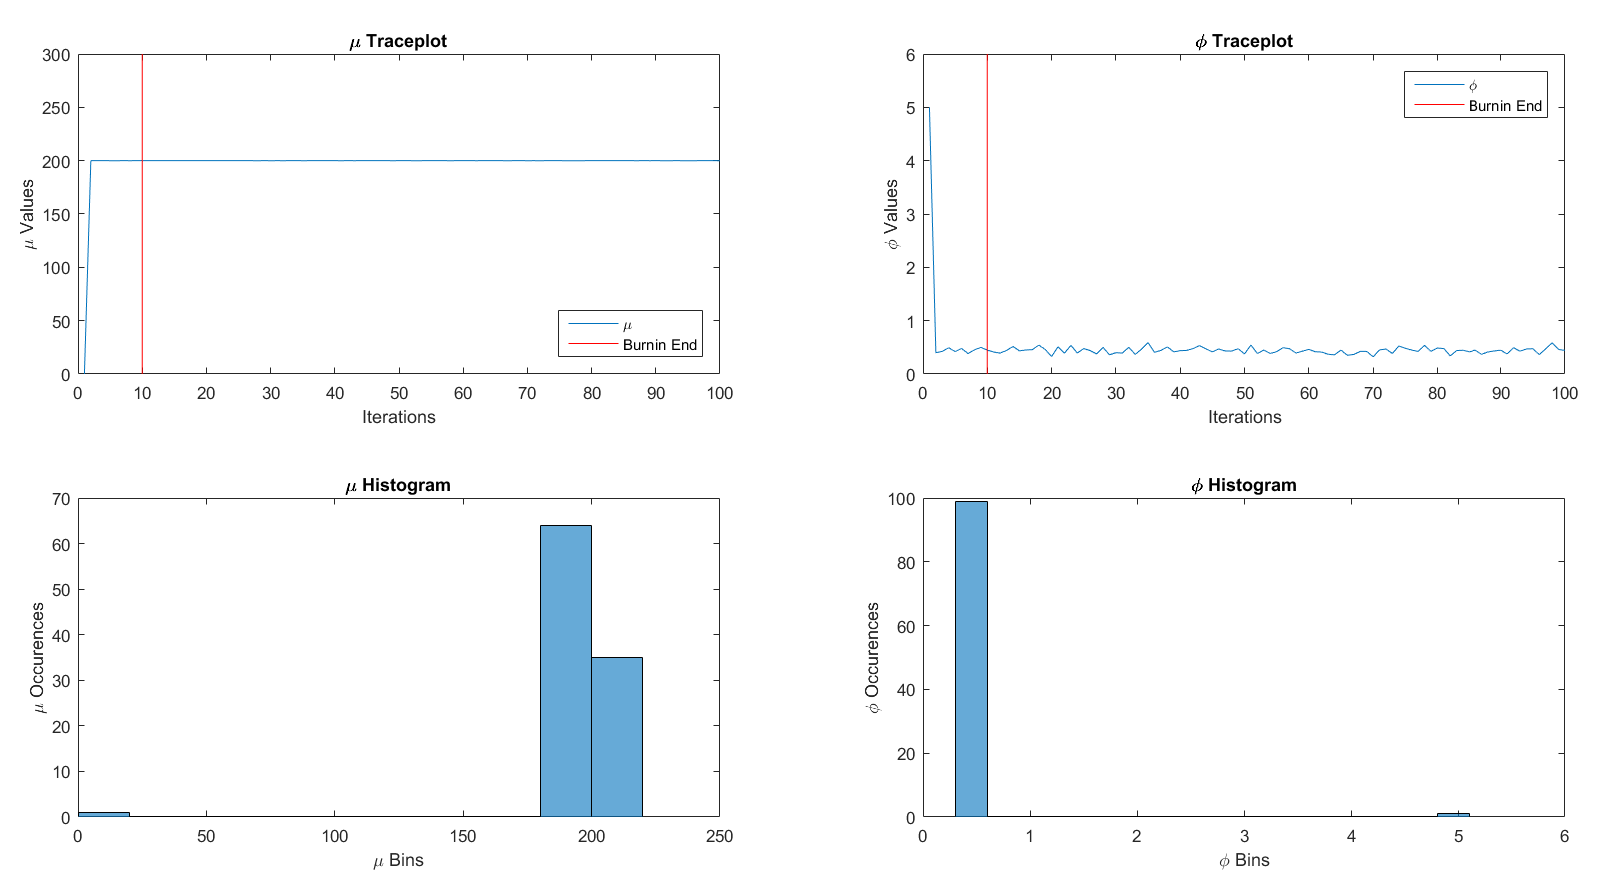
\includegraphics[scale = 0.4]{HW3_Part6} \\
\lstinputlisting{HW3Gibbs.m}
\end{homeworkProblem}
\pagebreak
\begin{homeworkProblem}
\begin{align*}
x_i &-Bin(N, p) \\
I(p) &= E([\frac{d}{d\theta}L(p|y)]^2|p) \\
I(p) &\propto E(\big[\frac{d}{dp}log(\frac{N}{x} p^x(1-p)^(N-x))\big]^2|p) \\
I(p) &\propto E(\big[\frac{d}{dp}xlog(p)+(N-x)log(1-p)\big]^2|p) \\
I(p) &\propto E(\bigg[\frac{x}{p} - \frac{n-x}{1-p}\bigg]^2|p) \\
I(p) &\propto E(\bigg[\frac{x^2}{p^2} 
	- 2\frac{x}{p}\bigg(\frac{n-x}{1-p}\bigg) 
	+ \bigg(\frac{n-x}{1-p}\bigg)^2 \bigg]|p) \\
I(p) &\propto E(\bigg[\frac{x^2}{p^2} 
	-\bigg(\frac{2nx-2x^2}{p(1-p)}\bigg) 
	+ \bigg(\frac{n-x}{1-p}\bigg)^2 \bigg]|p) \\
I(p) &\propto E(\bigg[\frac{x^2(1-p)^2 - 2(p(1-p)x(n-x)) + p^2(n-x)^2}{p^2(1-p)^2}\bigg]|p) \\
I(p) &\propto E(\bigg[\frac{p^2x^2-2px^2+x^2 - 
	2(pxn -px^2 - p^2xn+p^2x^2) + 
	p^2n^2-2nxp^2 +p^2x^2}{p^2(1-p)^2}\bigg]|p) \\
I(p) &\propto E(\bigg[\frac{x^2 - 2pxn + p^2n^2}{p^2(1-p)^2}\bigg]|p) \\
I(p) &\propto \sum_i\bigg[\frac{x^2 - 2pxn + p^2n^2}{p^2(1-p)^2}\bigg]
	\bigg[\frac{n}{x}p^x (1-p)^{n-x}\bigg]\\
I(p) &\propto \bigg[\frac{E(x^2) - 2pnE(x) + p^2n^2E(1)}{p^2(1-p)^2}\bigg]\\
Var(x) &= E[x^2] - (E[X])^2 \rightarrow E[x^2] = Var(x) + (E[X])^2 \\
E[x^2] &= Var(x) + (E[X])^2 = np(1-p) + n^2p^2 \\
E[x] &= np \\
E[1] &= 1 \\
I(p) &\propto \bigg[\frac{E(x^2) - 2pnE(x) + p^2n^2E(1)}{p^2(1-p)^2}\bigg]\\
I(p) &\propto \bigg[\frac{np(1-p) + n^2p^2 - 2p^2n^2 + p^2n^2}{p^2(1-p)^2}\bigg]\\
I(p) &\propto \bigg[\frac{np(1-p)}{p^2(1-p)^2}\bigg] = \bigg[\frac{n}{p(1-p)}\bigg]\\
p(p) &= I(p)^{1/2} = \bigg[\frac{n}{p(1-p)}\bigg]^{1/2} =\bigg[\frac{\sqrt{n}}{\sqrt{p(1-p)}}\bigg]\\
p &- Beta(1/2, 1/2) \rightarrow p(p) = (p^{-1/2}(1-p)^{-1/2}) * 
	\frac{\Gamma(1/2+1/2)}{\Gamma(1/2)\Gamma(1/2)} = (p^{-1/2}(1-p)^{-1/2}) * \frac{1}{\pi}\\
p(p) &= \bigg[\frac{\sqrt{n}}{\sqrt{p(1-p)}}\bigg] * \frac{1}{\sqrt{n}\pi}\\ \\
p &- Beta(\frac{1}{2}, \frac{1}{2})
\end{align*}
\end{homeworkProblem}
\end{document}
